\def \Subject {گام سوم}

% \def \Session {2}
% \setcounter{chapter}{\Session}

\section{\Subject}

\begin{itemize}
\item 
{
الفبای منبع در حالت ذکر شده چیست؟
همان طور که در تصویر مشخص است، 
\(y\)
از اعداد اعشاری تا 4 رقم اعشار تشکیل شده است.

  \begin{figure}[h!]
    \centering
    \makebox[\textwidth][c]{%
    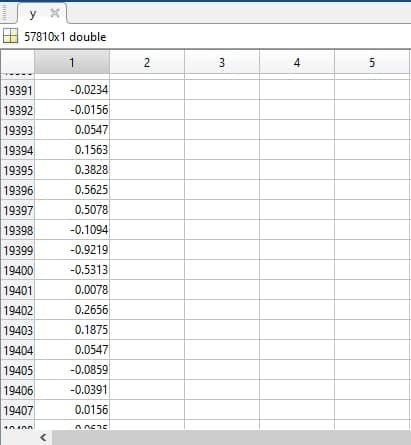
\includegraphics[height=0.5\textheight,width=0.7\textwidth]{images/y.jpg}%
    }
\end{figure}
}
\item  
{
سرعت تولید سمبل در منبع ذکر شده چه مقدار است ؟

\null \hfill $ \rightarrow t = \dfrac{|y|}{F_s} $ 
\null \hfill $ F_s = \dfrac{|y|}{t} $ \\

می دانیم که طول 
\(y\)
برابر با 
\(57810\)
است و مقدار 
\(F_s\)
را نیز در دست داریم، پس با استفاده از روابط بالا 
\(t = 5.2435\)
به دست می آید که با توجه به خود فایل عدد به دست آمده درست است.
}
\item 
{
اگر به همان فایل  
\(handle\)
گوش کنید شما چنین
قطعی در صدا نمی یابید. چرا؟ چرا در هنگام تماشای یک فایل ویدئویی با این که تنها  ۲۰تا  ۳۰فریم در ثانیه
پخش می شود، ولی شما هیچ گونه گسستگی در فیلم مشاهده نمی کنید؟
با توجه به قضیه 

اگر از یک سیگنال باند محدود، با دو برابر نرخ نایکویست نمونه برداری کنیم، می توانیم به
طور کامل از روی نمونه ها سیگنال پیوسته را بازیابی کنیم
پس اگر نرخ نمونه برداری 
\(2\)
برابر 
\(f_m_a_x\)
باشد، بدونه هیچ گونه گسستگی شنیده می شود.
}
\end{itemize}